% !TEX root = ../swputhesis.tex
\chapter{相关技术及理论介绍:感知像素级的图像全景分割方法}
\section{方法引述}
随着计算机技术的不断创新和突破,语义和实例分割领域得到了显著发展。全景分割作为语义和实例分割的综合应用,具有更深入理解和处理图像的能力,可以实现对像素级别的标签预测和更准确的场景分割。随着摄像机、数码相机和图像扫描仪的广泛应用,提供了更多的二维RGB图像数据资源,为全景分割提供了良好的基础。大多数研究者认为全景分割是处理二维RGB图像最佳的方法。

如今,在实时场景处理和精准预测等领域,普遍选择全景分割技术,例如自动驾驶系统。通过全景分割方法,可以提高图像分割的效率和准确性。为了降低全景分割的计算复杂度,可以设计自上而下的双阶段分割模型,并且在单阶段目标检测方面采用自上而下的单阶段分割模型,但需要消除生成区域的阶段。由于预测实例掩码和计算融合启发式的计算量较大,可以通过全景分割的方式将像素密集的自定义分类任务转化为更简化的形式。此外,在非最大抑制重叠的过程中,需要直接还原残留的密集边界提案。通过直接还原实例掩码,无需采样和处理聚类特征,可以减少全景分割的计算量。在骨干网络中,多分支的ResNRT-FPN网络包含多种不同维度的信息内容,通过融合多分支全景分支的方式生成感知全景实例的分数,从而解决了不同区域重叠的问题。与双阶段全景分割进行对比分析后发现,利用单阶段网络结构可以有效提高推理网络的效率,解决了融合冲突的问题,但会降低全景分割的质量。

为了在提高全景分割网络推理效率和质量方面取得成功,本研究设计了一种基于感知像素级实例掩码的单阶段网络架构。该网络以扩展FCOS目标检测器的方式来获得输出网络,从而生成目标检测、语义和全景三种分支结构。其中语义和全景分支的输出网络通过计算像素的乘积来预测全景分割。通过端到端的学习,可以防止启发式融合冲突的出现。通过感知像素级实例掩码的方法,可以有效降低大尺度物体边缘中心的偏移困难,并解决夸大分割大尺寸物体而无法有效分割小尺寸物体的问题。在本章节中,介绍了一种单阶段全景分割网络,它通过扩展FCOS目标检测器来实现输出网络,并生成目标检测、语义和全景三种分支结构。语义和全景分支的输出网络基于像素乘积计算来预测全景分割。该方法的设计目的是以高效简单的方式实现全景分割,并构建适用于实际应用场景的布局思路。通过本方法的研究,旨在平衡全景分割网络推理效率和质量的提升。为验证本方法的优势,本文在Cityscapes公开标准数据集上与当前主流的全景分割方法进行了比较,并分析了本方法在分割性能上的优势。

\section{方法流程}
在本节中,着重讨论了ResNet-FPN多尺度编码网络的特征提取能力,并详细介绍了FCOS基本结构及其扩展输出。通过采用语义和全景分支的方法,可以解码网络的特征,并使用全景分支来有效地预测每个像素偏移到实例中心的位置\cite{li2017fully}。\cref*{fig1}展示了整体网络架构的示意图。

\begin{figure}[!h] %h表示就在此处插入。
    \centering % 居中
    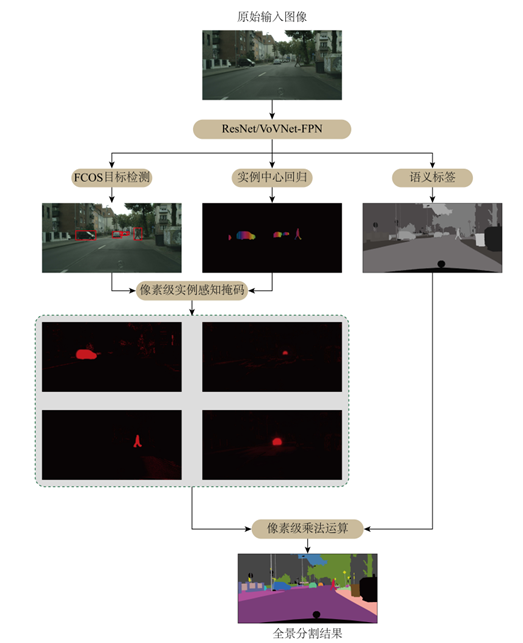
\includegraphics[scale=0.8]{fig/chap2/图片1.png} %在tex所在文件夹下面创建一个名为figs的文件夹,并把所有要用的照片放这里。当然你也可以选择使用绝对路径。
    \caption{全景分割网络架构}
    \label{fig1} % 为每个图片设置一个标识
    \end{figure}



\section{网络整体架构}
ResNet50网络主要用于提取输入图像的多尺度特征信息。在整个网络中,本文使用ResNet50作为主干网络,其主要功能是通过层级的卷积操作来提取输入图像的特征。同时,我们在网络的不同分支结构中获得了五个级别的特征图。

在目标检测分支中,我们使用了FCOS目标检测器来生成实例中心和感知像素级实例掩码。这个分支的主要目标是对输入图像进行目标检测,识别目标的位置和类别,并生成实例级别的掩码信息。

另一方面,语义分支的作用是为全景分支提供语义标签。语义分支利用网络的特征图来预测图像中每个像素点的语义类别,以提供更丰富的语义信息。

全景分割网络的输出是通过计算语义分支和全景分支之间的像素乘积得到的。这种方式降低了启发式融合冲突的可能性,同时减少了模型的计算量。通过融合语义信息和全景分支的输出,我们可以获得更精确的全景分割结果。

\subsection{特征提取网络}
在本节中,我们借鉴了FCOS目标检测器的思想,通过特征提取网络来获取多尺度的特征信息。我们将主干网络与金字塔特征网络结构相结合,其中主干网络采用了ResNet50-FPN架构。ResNet50-FPN由卷积块和恒等块组成。卷积块的输出和输入维度不同,无法直接连接,其主要作用是调整网络的维度。而恒等块的输出和输入维度相同,通过连续串联的方式可以增加网络的深度,有助于提取深层次的特征。
我们的网络采用了主干网络与金字塔特征网络结合的多尺度特征表示形式,旨在减少主干网络的计算负担。我们将输出特征图的通道数设置为128,具体的网络结构请参考\cref*{fig2}。

\begin{figure}[!h] %h表示就在此处插入。
    \centering % 居中
    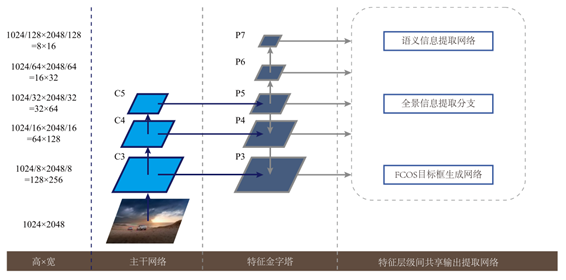
\includegraphics[scale=0.8]{fig/chap2/图片2.png} %在tex所在文件夹下面创建一个名为figs的文件夹,并把所有要用的照片放这里。当然你也可以选择使用绝对路径。
    \caption{特征提取图}
    \label{fig2} % 为每个图片设置一个标识
    \end{figure}

\subsection{分支网络}

\begin{figure}[!h] %h表示就在此处插入。
    \centering % 居中
    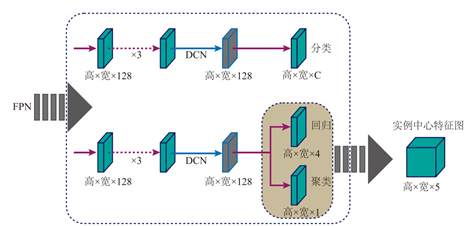
\includegraphics[scale=0.8]{fig/chap2/图片3.png} %在tex所在文件夹下面创建一个名为figs的文件夹,并把所有要用的照片放这里。当然你也可以选择使用绝对路径。
    \caption{分支网络图}
    \label{fig3} % 为每个图片设置一个标识
    \end{figure}
解码多尺度特征的网络主要由ResNet50-FPN组成,用于扩展特征提取网络的输出。本研究采用全卷积和无锚点的检测器来进行目标检测。FCOS在输出图像中对每个像素点的实例类别和中心进行有效预测,从而实现密集像素分类的集成和处理。这种方法有效降低了计算锚点目标和调整超参数的难度,减轻了模型训练的复杂性,并提高了推理效率。在该检测器中,通过五层融合的方式预测多尺度特征。\cref*{fig3}详细展示了该网络中预测层的三个输出。


其中,第一个输出被称为分类输出,其尺寸为H×W×C,其中H和W表示特征图的高度和宽度,C表示类别数。通过公式转换,可以将特征图上的像素位置(x ̂,y ̂)转换为输入图像中对应像素位置(x,y),其中s表示缩放比例。

\begin{equation}
    (x, y)=\left\{\left\lfloor\frac{s}{2}\right\rfloor+\widehat{x} \mathrm{~S},\left\lfloor\frac{s}{2}\right\rfloor+\widehat{x} \mathrm{~S}\right\}
    \label{eqk2}
    \end{equation}

\subsubsection{语义分支网络}
本研究提出的语义分支结构是一种轻量级结构,如图\cref*{fig4},它可以接收特征提取网络的多尺度特征,并且采集的特征图大小仅为原始图像的八分之一。采集的特征图经过特征拼接,将多尺度特征图的通道数扩展到640。接下来,使用金字塔池化模块来收集来自不同尺度的远程信息。首先,通过四个并行的平均池化操作生成四个尺度不同的特征图,它们的尺度分别是[1×1×640]、[2×2×640]、[4×4×640]和[8×8×640]。然后,将金字塔池化模块的输出和输入特征图进行拼接,经过1×1卷积核的作用,将融合特征图的通道数扩展到128。接着,通过三个大小为3×3的卷积核,进一步扩展特征的通道数到128,最终生成语义分支的信息。

\begin{figure}[!h] %h表示就在此处插入。
    \centering % 居中
    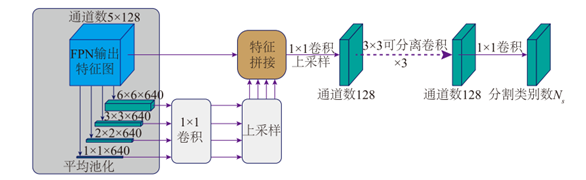
\includegraphics[scale=0.8]{fig/chap2/图片4.png} %在tex所在文件夹下面创建一个名为figs的文件夹,并把所有要用的照片放这里。当然你也可以选择使用绝对路径。
    \caption{语义分割网络}
    \label{fig4} % 为每个图片设置一个标识
    \end{figure}

\subsubsection{全景分支网络}
本研究提出了一种全新的全景分支网络,旨在实现语义分割和生成感知像素级实例掩码。该网络通过计算像素乘积的方式输出语义分支,从而获得全景分割的输出结果。我们采用端对端的方式对全景分支网络进行训练和推理学习,以确保网络的一致性和准确性。
\begin{figure}[!h] %h表示就在此处插入。
    \centering % 居中
    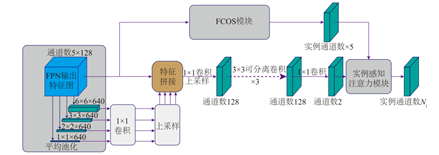
\includegraphics[scale=0.8]{fig/chap2/图片5.png} %在tex所在文件夹下面创建一个名为figs的文件夹,并把所有要用的照片放这里。当然你也可以选择使用绝对路径。
    \caption{全景分割网络}
    \label{fig5} % 为每个图片设置一个标识
    \end{figure}

通过预测实例像素的偏移量来计算实例掩码是我们的关注重点。我们设计了全景分支结构,与语义分支结构非常相似,具体架构可参考\cref*{fig5}。全景分支结构生成了一个双通道的输出特征图,使用3x3的卷积核。这个特征图表示了像素相对于实例中心的偏移量在x轴和y轴上的值。由于对象在图像中的尺度是不同的,不同尺度的对象与实例中心的距离存在不同的比例关系。对于大尺度的对象,远离实例中心的边缘像素的偏移量很难准确预测。为了解决这个问题,我们采用了感知不同实例像素级掩码的方法,以降低计算边缘像素偏移量的难度。通过预测像素偏移量、计算对象尺度和真实实例中心之间的关系,我们可以得到感知实例像素级掩码。全景分支网络的输出可以预测像素的偏移量。具体而言,我们使用二维高斯函数(均值位于边界框的中心,标准差由其大小给出)将全景分支预测的偏移量转化为像素属于该实例的概率:

\begin{equation}
    M\left(l_i, l_j\right)=\exp \left(-\frac{\left(l_i+d_i-x_k\right)^2}{w^2}-\frac{\left(l_j+d_j-y_k\right)^2}{h^2}\right)
    \end{equation}

当预测的实例中心位置与真实实例中心偏离时,属于该实例的概率会在物体边缘处逐渐衰减。为了生成实例掩码,本研究采用了像素级实例感知掩码作为语义分支的滤波器。通过对语义分支的掩码和像素级实例感知掩码进行逐像素的乘法运算,我们得到了最终的全景分割分数。这种逐像素的乘法运算将语义信息和实例感知信息相结合,以提高对实例边缘的分割准确性和细节表达能力。



其中$ C_k\left(l_{\mathrm{i}}, \mathrm{l}_{\mathrm{j}}\right) $
表示点$ \left(l_{\mathrm{i}}, \mathrm{l}_{\mathrm{j}}\right) $所在位置的语义分支信息。
